\documentclass[11pt, a4paper]{article}
\usepackage{lmodern}
\usepackage[utf8]{inputenc}
\usepackage[czech]{babel}
\usepackage{hyperref}
\usepackage{graphicx}
\usepackage{caption}
\usepackage{pdfpages}
\usepackage{geometry}

\begin{document}
%
% Titulni strana
%
\begin{titlepage}
\centerline{
\includegraphics[width=6cm]{zculogo.png}}
\vspace*{50px}
\begin{center}
{\LARGE\bf\noindent KIV/PC Semestrální práce}\\
(Optimalizace funkce genetickým algoritmem)
\vspace*{40px}

Pavel Třeštík \\
 (A17B0380P)\\
\vspace*{\fill}
\hspace*{\fill} \today \\
\end{center}
\end{titlepage}
\newpage
%
% Obsah
%
\pagenumbering{arabic}
\tableofcontents
\newpage
%
%
%
%
% ZAČÁTEK
%
%
% Zadání
%
\section{Zadání}
%
% Zjednodušené zadání
%
\subsection{Zjednodušené zadání}
Cílem je napsat přenositelnou konzolovou aplikaci, která bude hledat extrém funkce pomocí genetického alrgoritmu.\\
Základní princip genetickoho algoritmu:
\begin{enumerate}
  \item Náhodně vytvoříme několik různých řešení zadané úlohy -- jedinců.
  \item Provedeme křížení jedinců.
  \item Náhodně zmutujeme malý počet jedinců.
  \item Ověříme, jak dobře každý jedinec řeší náš problém tak, že pro každého získáme hodnotu fitness funkce.
  \item Vytvoříme novou generaci.
  \item Opakujeme kroky 2 až 5.
\end{enumerate}
\subsection{Parametry programu}
Aplikace bude přijímat z příkazové řádky 2 povinné argumenty:
\begin{itemize}
  \item jméno souboru, ve kterém jsou metadata o testované funkci,
  \item počet generací, které mají být provedeny.
\end{itemize}
Program bude také přijímat jeden nepovinný argument:
\begin{itemize}
  \item \textbf{-m} \it procento mutací (0-100).
\end{itemize}
Pokud nebudou na příkazové řádce uvedeny alespoň dva argumenty, vypište chybové hlášení a stručný návod k použití programu (v angličtině).
\subsection{Popis programu}
\subsubsection{Mapování genu}
Pro mapování genu se doporučuje použít dále uvedený způsob:
\begin{itemize}
  \item Pro celá čísla použijte jejich binární zápis.
  \item Pro reálná čísla použijte konkrétní hodnoty daných proměnných.
\end{itemize}
\paragraph{Křížení}
Křížení dvou potomků se realizuje pro každou skupinu genů takto:
\begin{itemize}
  \item Pro binární zápis celého čísla kombinujte části genů rodičů (viz Obrázek 1). Hranici bloků vyrábějte vždy náhodně, ale tak, aby sapdla mezi bity kódující interval uvedený u proměnné.
  \item Pro hodnotu reálného čísla vypočítejte pro potomka novou hodnotu jako aritmetický průměr hodnot rodičů.
\end{itemize}
\begin{figure}[h]
  \includegraphics{one_point_crossover.jpg}
  \caption{Ukázka tvorby nových potomků zeleného a modrého rodiče\\Zdroj: www.tutorialspoint.com}
  \label{fig:one_point}
\end{figure}
\paragraph{Mutace}
Mutaci genotypu provádějte následujícím způsobem. Podle parametru z příkazové řádky \textbf{-m} vyberte určitou část z populace, kterým náhodně upravíte část genů. Část binární reprezentace celého čísla náhodně přepíšete nulami a jedničkami. U reálného čísla, reprezentovaného hodnoutou vygenerujete náhodně nové číslo z uvedeného intervalu. U mutovaného potomka však vždy upravte jen jednu skupinu genů.\\\\Dejte však pozor ať mutací neponičíte své nejlepší jedince.
\subsection{Výstup}
Výsledkem programu budou dva textové soubory (gen.txt a val.txt), ve kterých bude souhrn průběhu hledání optima. Protože celý proces může být velice časově náročný, tyto soubrory tvořte průběžně.
\subsection{Originální zadání}
https://www.kiv.zcu.cz/studies/predmety/pc/doc/work/sw2018-01.pdf
\newpage
%
% Teoretický rozbor
%
\section{Analýza úlohy}
V první řadě program bude muset načíst intervaly ze souboru s metadaty. Program bude číst soubor po řádkách a pokud načte řádku, která začíná na "\#\_(", bude vědět, že se jedná o řádku, která udává interval. Z této řádky následně získá potřebné údaje intervalu, tj. jeho spodní a horní hranici a typ.\par
V další části už program začne pracovat na geneticém algoritmu. Jelikož už má intervaly, může vytvořit první generaci, jejíž jedinci mají kompletně náhodné koeficienty z daných intervalů.\par
Aby program mohl vytvořit další generace, bude potřebovat zjistit fitness hodnotu každého jedince. Protože se jedná o hledání extrému funkce, tak hodnotu fitness funkce bude udávat extrém funkce, daného jedince. K počítání extrému je nám poskytnut program, který extrém vypočte a proto se fitness bude počítat úpravou souboru s metadaty a voláním poskytnutého programu.\par
Před vytvářením další generace, program seřadí generaci podle fitness hodnoty.\par
V této fázi program může vytvářet další generaci. Další generace se vytvoří tak, že jedinci z lepší části generace se kříží mezi sebou a vytváří tím nové jedince. Jedinci se kříží způsobem uvedeným v zadání. To je:
\begin{itemize}
  \item z reálných koeficientů se udělá aritmetický průměr,
  \item z celých koeficientů se prohodí část jejich binárního zápisu.
\end{itemize}
U prvního případu není problém, protože aritemetický průměr dvou čísel z intervalu bude také ležet v tomto intervalu. Problém nastává u celých čísel, kdy při prohození pouze určitého počtu bitů může nastat situace, kde nový koeficient bude mimo interval. Jelikož ale neznám žádný algoritmus, který by zajišťoval, že po prohození určitého bloku binárního zápisu čísel, výsledek bude také v intervalu původních čísel, tak se pravděpodobně budu muset spolehnout na brute-force přístup. To znamená, že algoritmus bude muset testovat prohození každé možné délky bloku čísla a také by měl vzít v potaz, aby vůbec nastala nějáká změna v hodnotách (aby neprohodil pouze blok o takové velikosti, kde jsou bity shodné, tudíž by nenastala žádná změna v koeficientu).\par
Ačkoliv reálné koeficienty při křížení davají pouze jeden výsledek, prohazování bloků celých čísel dá výsledky dva, čímž při křížení dvou jedinců získáme dva nové jedince. Z tohoto důvodu se horší část generace bude přepisovat novými jedinci, získanými křížením lepší poloviny generace.\par
V předposledním kroku se provede mutace generace. Mutace jedince se provádí pouze na jedné skupině genů. Na základě typu genu, který se mutuje, se mutace provádí, jak je popsáno v zadání. Tedy reálnému koeficientu se vygeneruje nové náhodné číslo z daného intervalu a celému koeficientu se prohodí náhodný počet bitů jedničkami za nuly a opačně. Podobně jako u křížení ale u mutace celého koeficientu vzniká problém, zda nové číslo bude patřit do náležitého intervalu. Narozdíl od křížení se zde neprohazují pouze jednotné bloky čísla, ale jednotlivé bity nezávisle na pozici. Proto algortimus, který bude zajišťovat, aby nové číslo patřilo do intervalu, nemusí být vyloženě brute-force. Pokud nové číslo přeshuje horní hranici intervalu, tak vzhledem k tomu, že můžeme změnit libovolný bit, jednoduše zmutovanému číslu změníme nejbližší bit s výšší hodnotou, než je rozdíl nového čísla a horní hranice intervalu. Podobně bude fungovat i dolní hranice intervalu, ale místo aby se nejbližší vyšší bit přepisoval na 0, tak se bude nejbližší bit s vyšší hodnotou, než rozdíl dolní hranice intervalu a nového čísla, přepisovat na 1.\par
V poslední řadě zbývá akorát udělat výstup do souborů. Do gen.txt se po každé nové generaci zapíše její pořadí a její nejlepší jedinec, resp. jeho extrém (fitness) a  koeficienty. Do val.txt se po každé generaci zapíší hodnoty extrémů všech jedinců generace a jejich koeficienty.
\newpage
%
% Implementace
%
\section{Popis implementace}
\subsection{Obecný popis}
Program se skládá ze dvou souborů s příponou .h (specimen.h a generation.h) a tří souborů s příponou .c (specimen.c, generation.c a main.c).\par
\subsection{Podrobné popisy}
\subsubsection{specimen.h}
\textbf{specimen.h} obsahuje dvě globální proměnné, *calc\_func, která uchovává řetězec na spuštění programu pro spočítání extrému a *meta\_nace, která uchovává pouze název souboru s metadaty (bez cesty).\par
Dále obsahuje tři struktury (viz Obrázek 2).\\\\Struktura \textbf{coef} ukládá všechny koeficienty jedince.\\\\Struktura \textbf{specimen} (struktura jedince) obsahuje jedincovo id, ext (extrém = hodnota fitness) a *coef - pointer na pole koeficientů jedince.\\\\Struktura \textbf{interval} s proměnými: typ - typ intervalu, bot - spodní hranice intervalu, top - horní hranice intervalu.
\begin{figure}[h]
  \includegraphics{spec_structs.png}
  \caption{Struktury z hlavičkového souboru specimen.h}
  \label{fig:specimen_structs}
\end{figure}\\
V poslední řadě specimen.h obsahuje prototypy (viz Obrázek 3). Prototyp create\_specimen slouží k vytvoření jednice. Get\_extreme používaný k získání extrému jedince - neboli jeho fitness hodnoty. Crossbreed kříží dva jedince. Mutate mutuje předaného jedince.
\begin{figure}[h]
  \includegraphics{spec_prots.png}
  \caption{Prototypy z hlavičkového souboru specimen.h}
  \label{fig:specimen_prots}
\end{figure}\\
\subsubsection{specimen.c}
Souboru specimen.h náleží \textbf{specimen.c}, jehož funkce následují.\\\\Funkce \textbf{create\_specimen}, vzhledem k tomu, že důležité věci pro jedince jsou předány parametry, tak funkce pouze alokuje na tyto struktury paměť.\\\\Funkce \textbf{get\_extreme} zjišťuje extrém předaného jedince. Funkce nepočítá nic sama o sobě, pouze upravuje zdrojový soubor a volá poskytnutou funkci, která extrém spočítá.\\\\Funkce \textbf{crossbreed} zkříží skupiny genů rodičů a vytvoří tak 2 nové jedince. Pokud je křížený gen reálné číslo funkce pouze udělá jeho aritmetický průměr a výsledek přiřadí oběma potomkům. Pokud se ale jedná o celé číslo, funkce ho nejdříve převede na binární zápis, protože ve stuktuře "coef" je celé číslo reprezentováno hodnoutou a né binárním zápisem, jak je doporučeno v zadání. Během tohoto převodu funkce navíc získá pozici nejvýznamnějšího bitu převáděného čísla. Následně zkouší prohazovat bloky o zvětšující se velikosti od nejvýznamnějšího získaného bitu do nejméně významného bitu. Bohužel, jak předpokládáno v analýze, funkce toto dělá pro každou velikost bloků, kdy nastane změna (tzn. bity na konečné pozici bloků se neshodují) tudíž se jedná a použití burte-force. Pokud není možné prohodit žádné bity, funkce pouze prohodí původní hodnoty celých čísel. Pokud je více než 1 možnost funkce náhodně jednu zvolí.\\\\Funkce \textbf{mutate} zmutuje pouze jednu skupinu genů předaného jedince. Funkce tedy náhoně vybere jeden koeficient. Pokud je vybraný koeficient realné číslo, funkce vygeneruje nové náhodné číslo z náležitého intervalu. Pokud je koeficient celé číslo, funkce převede koeficient na binární zápis přičemž, stejně jako u crossbreed uloží pozici nejvýznamnějšího bitu koeficientu. Program následně vybere náhodný počet pozic, ovšem maximálně polovinu genu, které zneguje. Pokud zmutovaný koeficient přesahuje hranici intervalu, funkce zneguje bit s nejbližší vyšší hodnout než je rozdíl horní hranice intervalu a výsledku. Pokud je číslo menší než spodní hranice intervalu, tak program neguje bity od nejméně významné bitu, dokud se číslo v intervalu nenachází.\\\par
\subsubsection{generation.h}
Soubor \textbf{geneneration.h}. Obsahuje jednu globální proměnnou - mutation\_rate - procento mutací.\par
Tento soubor má jednu strukturu a tou je generation (viz. Obrázek 4). Generation obsahuje gen\_num udávájící o kolikátou generaci se jedná a species - pole jedinců v generaci.
\begin{figure}[h]
  \includegraphics{gen_struct.png}
  \caption{Struktura z hlavičkového souboru generation.h}
  \label{fig:gen_struct}
\end{figure}\\
Prototypy generation.h (viz Obrázek 5).
\begin{figure}[h]
  \includegraphics{gen_prots.png}
  \caption{Prototypy z hlavičkového souboru generation.h}
  \label{fig:gen_prots}
\end{figure}\\
\subsubsection{generation.c}
Souboru generation.h náleží \textbf{generation.c} s následujícími funkcemi.\\\\Funkce \textbf{create\_first\_generation} vytvoří novou generaci s kompletně náhodnými koeficienty jedinců. Nejdříve alokuje paměť pro koeficenty všech jedinců. Následně generuje náhodné hodnoty koeficientů pro každého jedince. Spočítá extrémy všech jedinců a seřadí je.\\\\
Funkce \textbf{next\_generation} vytváří další generaci. Nejdříve vygeneruje dvě pole uchovávající indexy lepší poloviny generace, které budou tvořit páry, které se budou mezi sebou křížit. Následně se provádí křížení těchto párů. Po křížení se generace mutuje. Na rozdíl od zadání je ale možné mutovat pouze 5 až 45 procent generace. To je z důvodu, aby v každé generaci nastala alespoň nějáká změna (proto minimálně 5 procent mutace pro každou generaci) a 45 procent je maximum proto, aby mutace nepoškodily 5\% nejlepší jedinců a ani nové jedince vytvořené křížením, kteří tvoří polovinu generace. Nakonec funkce spočte extrémy a seřadí generaci.\\\\
Funkce \textbf{calc\_generation\_extremes} pouze volá funkci get\_extreme pro každého jedince generace.\\\\
Funkce \textbf{print\_generation} vypisuje do konzole nejlepšího a nejhoršího jedince proběhlé generace.\\\\
Funkce \textbf{free\_gen} uvolňuje pamět coeficientů generace.\\\\
Funkce \textbf{print\_gen\_to\_file} vypíše do souboru gen.txt číslo generace a jejího nejlepšího jedince.\\\\
Funkce \textbf{print\_val\_to\_file} vypšíe do souboru val.txt extrémy všech jedinců a jejich koeficienty.\\\\
Funkce \textbf{print\_files} volá print\_gen\_to\_file a print\_val\_to\_file, aby nebylo třeba je volat zvlášť (ovšem aby to bylo možné).\\\\
Mimo tyto funkce generation.c ještě obsahuje funkci \textbf{compare} sloužící k seřazení jedinců v generaci.\\\\
\subsubsection{main.c}
Soubor \textbf{main.c} obstarává obsluhu programu. Obsahuje následující funkce.\\\\
Funkce \textbf{prepare\_func\_file} připravý soubor s metadaty a vytvoří jeho kopii v pracovním adresáři programu, s kterou poté bude pracovat.\\\\
Funkce \textbf{init\_intervals} inicializuje intervaly ze souboru, způsobem popasným v analýze.\\\\
Funkce \textbf{help} vypíše do konzole nápovědu k použití programu.\\\\
Funkce \textbf{init} obstarává korektnost argumentů.\\\\
Funkce \textbf{run} provozuje celý program.\\\\
Funkce \textbf{shutdown} po doběhnutí programu uvolňuje paměť.\\\\
\newpage
%
% Uživatelská příručka
%
\section{Uživatelská příručka}
\subsection{Přeložení}
Program se přeloží zavoláním příkazu \textbf{make} na linuxu. Na Windows uživatel bude potřebovat prostředí umožňující volat make. K tomuto uživatel muže využít například Visual Studio nebo MinGW apod. (pro každé prostředí make funguje jinak!! Pro použití prostředí si přečtěte jeho dokumentaci!). \textbf{Předpokládané použití} pokud uživatel používá Visual Studio, musí přejmenovat poskytnutý makefile.win na pouze makefile a z příkazové řádky Visual Studia zavolat příkaz \textbf{nmake}. Pro MinGW uživatel musí stejným způsobem přejmenovat makefile.win a z příkazové řádky na pozici pracovního adresáře zavolat "disk:\textbackslash cesta\textbackslash k\textbackslash mingw32-make.exe"\par
\subsection{Spuštění a obsluha}
Po přeložení se vytvoří spustitelný soubor \textbf{gms} (resp. \textbf{gms.exe} pro Windows), který lze spustit způsobem \textbf{./gms [meta\_source\_file] [number\_of\_generations] -m [percent\_of\_mutations]}. První dva parametry jsou povinné. "-m" je nepovinný parametr, udávající jaké procento generace se zmutuje, při vytváření nové generace. Pokud je použit přepínač "-m" musí povinně být zadán čtvrtý parametr - procento generace, jaké bude zmutováno, v rozmezí 5 až 45. Pokud nejsou zadány alespoň 2 parametry nebo je použit nesprávný přepínač a nebo pokud je použit správný přepínač, ale nezadá se procento mutace (popřípadě je zadáno chybné procento mutace), program vypíše chybovou hlášku a nápovědu k použití (viz Obrázek 6). Uživatel také může zobrazit nápovědu z Obrázku 6 bez chybové hlášky použitím jediného parametru \textbf{-h} (příklad volání: \textbf{./gms -h}).
\begin{figure}[h]
  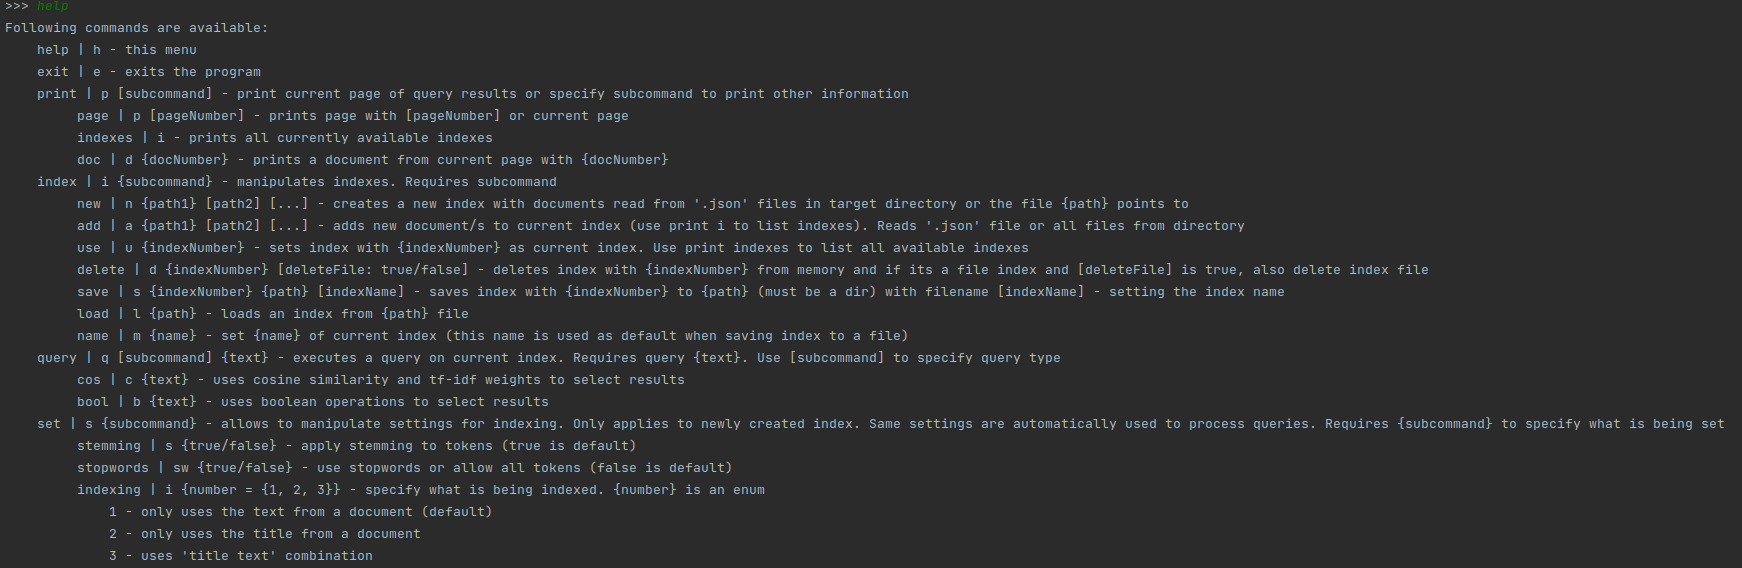
\includegraphics{help.png}
  \caption{Příklad nápovědy a chybového hlášení při spuštění programu, kdy je zadáno chybné procento mutace}
  \label{fig:help}
\end{figure}\\
Příklad správného spuštění programu a průběžného výstupu generace do konzole - Obrázek 7.
\begin{figure}[h]
  \includegraphics{run_ex.png}
  \caption{Příklad správného spuštění a průběžného výpisu}
  \label{fig:ex}
\end{figure}\\
\subsection{Výstupy}
Výstupy programu jsou dva textové soubory \textbf{gen.txt} a \textbf{val.txt}, které se tvoří průběžně během běhu programu. Mimo tyto soubory program také vypisuje informace o provedené generaci do konzole (viz Obrázek 7).\par
Soubory mají formát popsaný v originálním zadání. Příklad záznamu ze souboru gen.txt - Obrázek 8 a ze souboru val.txt - Obrázek 9.
\begin{figure}[h]
  \includegraphics{gen_out.png}
  \caption{Příklad posledních dvou záznamů gen.txt získaných voláním příkladového příkazu z Obrázku 7}
  \label{fig:gen_out}
\end{figure}
\begin{figure}[h]
  \includegraphics{val_out.png}
  \caption{Příklad posledních dvou záznamů val.txt získaných voláním příkladového příkazu z Obrázku 7}
  \label{fig:val_out}
\end{figure}
\clearpage
%
% Závěr
%
\section{Závěr}
Zadání program víceméně splňuje, ačkoliv má pár změn. Jedna změna je v ukládání celých čísel, kdy zadání doporučuje ukládat čísla v binární podobě, ale můj program je má uložené hodnotou. Druhá změna je rozsah procent mutací, kdy v zadání je naznačeno že procenta můžou být v rozsahu 0-100, ovšem zadání také říká, abychom si dali pozor, aby mutace neponičila nejlepší jedince. Vzhledem k tomu, že program provádí mutaci až po křížení jedinců, což znamená, že půlka nové generace jsou kříženci předchozí, tak jsem zvolil rozsah procent mutací 5-45. Pět procent z důvodu, aby se v každé generaci nějáký jednotlivec změnil, protože pokud by bylo procento mutací 0, po určitém počtu generací by se jednotlivci přestali zlepšovat a všichni by byli stejní. Čtyřicetpět je horní hranice proto, že nová generace je z poloviny tvořena kříženci a -5\% předpokládaných, aby se nemutovali nejlepší jedinci.\par
Na linuxu program probíhá rychle, tak rychle, že téměř není znát náročnost některých výpočtů a funkcí. Na Windows ovšem kompletně stejný program běží i více než deset krát pomaleji, což naznačuje, že některé části programu budou mít velkou výpočetní složitost nebo jsou z jiného důvodu velmi časově náročné na systému Windows.\par
Bylo by vhodnější prozkoumat, zda neexistují lepší algoritmy například na křížení celých čísel dvou jedinců, protože stávající algoritmus je ve své podstatě brute-force, tedy velmi výpočetně složitý. Také by chtělo vzít v potaz uložení některých proměnných (konkrétně celého čísla), protože pokud by bylo uloženo jako binární číslo, jak doporučuje zadání, ušetřilo by se značné množštví převodů celého čísla do binární podoby. V poslední řadě pravděpodobně poměrně náročný proces je zapisování dat do souborů, kdy proto aby soubory měly vyžadovaný formát, či aby se soubor změnil, jak je požadováno tak se musí přesouvat přes pomocný soubor. Tento proces je ale omezením jazyka a není k němu žádné výrazné vylepšení.\par
\end{document}
